\documentclass[11pt]{article}

\usepackage[utf8]{inputenc}
\usepackage{amsmath}
\usepackage{amssymb}
\usepackage{graphicx}
\usepackage{booktabs}
\usepackage{hyperref}
\usepackage[backend=biber,style=numeric-comp]{biblatex}

\addbibresource{bibliography.bib}

\title{Uncertainty-Aware Neural Surrogate for Parametric L-Bracket Stress Prediction}
\author{Anonymized for submission}
\date{}

\begin{document}
\maketitle

\begin{abstract}
% Phase 3: final abstract. Covers problem, reliability-layer contribution, headline calibration + OOD results.
\end{abstract}

\section{Introduction}
% Phase 1: motivate parametric L-bracket stress prediction and the need for a deployment-calibrated uncertainty layer. Positioning: the contribution is the reliability layer, not the surrogate.

\section{Related Work}
% Phase 2 pass will add full Related Work. Phase-1 placeholder below calls out
% only the two architectures that directly shape the surrogate choice in
% Methods; everything else (UQ methodology, CP, OOD for SciML) is added in
% Phase 2.
Graph neural networks are a natural fit for stress-field prediction on
unstructured FEA meshes because they act directly on the native
discretization without projecting onto a regular grid. Maurizi et
al.~\cite{maurizi2022gnn} demonstrate that mesh-based GNNs predict
displacement and stress fields on 2D solid-mechanics benchmarks to within a
few percent of the reference FEA solution. Pfaff et al.'s
MeshGraphNets~\cite{pfaff2021meshgraphnets} supply the
encoder--processor--decoder template with learned edge features that the
present work adopts (details in Methods~\S\,GNN architecture, Phase~1).

\section{Methods}

\subsection{Problem formulation}

We study an equal-arm symmetric L-bracket under a static shelf load, solved
as a two-dimensional plane-stress linear-elasticity problem. Let
$\Omega \subset \mathbb{R}^2$ denote the bracket cross-section in the $xy$
plane. With out-of-plane thickness $t = 8$~mm and in-plane extent
$A = B = 80$~mm, the aspect ratio $t/A = 1/10$ places the part in the
thin-plate regime, so plane stress (rather than plane strain or full 3D) is
the appropriate reduction. The governing equations are
\begin{equation}
  \nabla \cdot \boldsymbol{\sigma} = \boldsymbol{0}
  \quad \text{in } \Omega,
  \qquad
  \boldsymbol{\sigma} = \mathsf{C}:\boldsymbol{\varepsilon}(\boldsymbol{u}),
  \qquad
  \boldsymbol{\varepsilon} = \tfrac{1}{2}
    \bigl( \nabla \boldsymbol{u} + (\nabla \boldsymbol{u})^\top \bigr),
\end{equation}
with $\mathsf{C}$ the plane-stress isotropic-elasticity tensor and
$\boldsymbol{u}$ the unknown displacement field. Body forces are omitted:
under the calibrated applied load the self-weight contribution to peak
stress is $\sim 10^{-3}$ of the load-driven contribution, below the
discretization error introduced by mesh refinement.

\subsection{Geometry parameterization}

\begin{figure}[t]
  \centering
  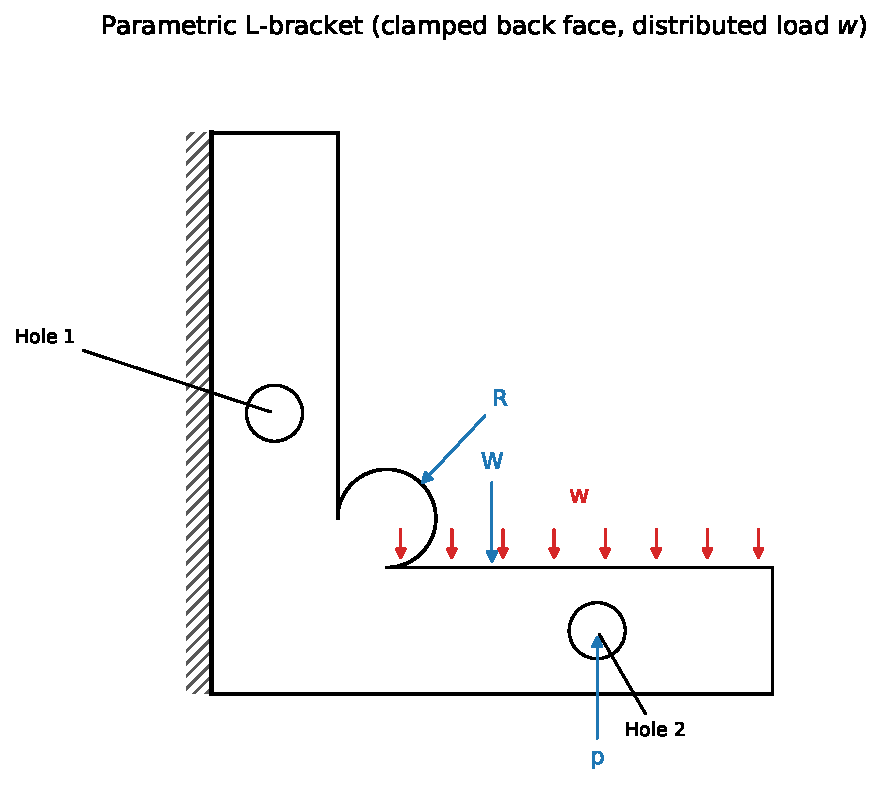
\includegraphics[width=0.60\linewidth]{figures/fig_geometry_schematic.pdf}
  \caption{Parametric L-bracket. Fixed dimensions: arm lengths $A = B =
    80$~mm, out-of-plane thickness $t = 8$~mm, hole diameter $D = 8$~mm.
    Three variable parameters: inside fillet radius $R$, Hole-2 position
    along the horizontal flange $p$, and flange width $W$. The back face
    of the vertical flange is clamped; a distributed traction $w$ acts
    downward on the top face of the horizontal flange.}
  \label{fig:geom}
\end{figure}

Three dimensions are exposed as free design parameters:
\begin{enumerate}
  \item $R$ — inside fillet radius at the concave corner.
  \item $p$ — $x$-position of Hole~2 along the centerline of the horizontal
    flange.
  \item $W$ — in-plane flange width, common to both arms.
\end{enumerate}
Parameter ranges were fixed by engineering inspection of limiting
geometries (too-sharp fillet, too-narrow flange, Hole~2 encroaching on the
fillet or the free tip):
\begin{equation}
  R \in [3.0, 10.0]~\text{mm},
  \quad
  p \in [42.0, 72.0]~\text{mm},
  \quad
  W \in [14.0, 24.0]~\text{mm}.
\end{equation}
All remaining dimensions are fixed by design intent. Hole~1 is centered on
the vertical flange at $y = 40$~mm from the top, providing a mounting
point whose location is invariant under the design sweep; Hole~2 has the
same bolt-clearance diameter $D = 8$~mm as Hole~1. The outside corner is
kept sharp: being on the compressive outer bend, it is not a
stress-concentrating feature and adding a second fillet parameter would
dilute the sensitivity analysis without mechanical justification. The
inside-fillet constraint $W + R \leq 34$~mm
(from $y_{\text{Hole 1}} - r_h - \text{clearance} \geq W + R$ with
$y_{\text{Hole 1}} = 40$~mm, $r_h = 4$~mm, clearance $= 2$~mm) binds the
joint upper corner of the sweep box and gives the LHS design a small
rejection rate that is absorbed by oversampling (Section~\ref{ssec:lhs}).

\subsection{Material model}

The bracket is modelled as a single homogeneous linear-elastic isotropic
material. AISI~304 annealed stainless steel is chosen as representative of
a thin shelf-bracket specification. Young's modulus and Poisson's ratio are
taken from the ASM Handbook~\cite{asm_handbook_vol1}:
$E = 193$~GPa, $\nu = 0.29$. The minimum specified yield strength
$\sigma_y = 205$~MPa is the ASTM A240 flat-product value for this
alloy~\cite{astm_a240}. These three constants fully determine the
plane-stress elasticity tensor. Plastic response is not modelled: the
load is calibrated so that the worst-case peak von~Mises stress reaches
$\sim 50\%$ of $\sigma_y$, keeping the full parametric sweep safely in the
elastic regime.

\subsection{Boundary conditions and loading}
\label{ssec:bcs}

A homogeneous Dirichlet condition $\boldsymbol{u} = \boldsymbol{0}$ is
applied on the back face of the vertical flange (the region $x = 0$,
$0 \leq y \leq A$). This idealizes a bracket rigidly mounted to a stiff
planar support; bolt-hole through-thickness contact mechanics are
deliberately omitted and Hole~1, although present as a geometric feature,
carries a traction-free boundary condition rather than a discrete
bolt-reaction force. This reduction is standard for screening-level
sizing analyses and localizes the modelling effort on the geometric
stress concentrators ($R$, holes) rather than on the fastener detail.

The loading models a shelf resting on the top face of the horizontal
flange. A constant downward traction
$\boldsymbol{t} = (0, -w)$~MPa acts on the segment
$W + R \leq x \leq B,\; y = W$. All remaining boundary segments (free tip,
horizontal-flange bottom, vertical-flange top, fillet arc, and both hole
perimeters) are traction-free.

The load magnitude $w$ is calibrated in a single preliminary run on the
worst-case sample $(R, p, W) = (3.0, 42.0, 14.0)$: a unit-load probe gives
peak von~Mises $119.8$~MPa, and the linearity of the elasticity operator
yields $w = 0.5\,\sigma_y / 119.8 = 0.8555$~MPa as the value that drives
the worst-case peak stress to exactly $0.5\,\sigma_y = 102.5$~MPa. The
same $w$ is used across all LHS samples, so the stress distribution
across the training set sweeps the full $\sim [50, 120]$~MPa elastic band
as $(R, p, W)$ vary.

\subsection{Finite-element discretization}

The problem is solved with FEniCSx~\cite{dokken_fenicsx} on unstructured
triangular meshes produced by Gmsh. Displacements are represented on a
Lagrange order-2 vector element (quadratic $T_6$ triangles), giving an
integration order sufficient to capture the quadratic stress distribution
through the flange thickness without mesh-doubling. Stresses are
recovered by differentiation and interpolated to a scalar Lagrange order-2
space; the von~Mises norm is formed pointwise as
$\sigma_{\mathrm{vM}} =
\sqrt{\sigma_{xx}^2 - \sigma_{xx}\sigma_{yy} + \sigma_{yy}^2
+ 3\sigma_{xy}^2}$, which is the correct plane-stress reduction of the
3D von~Mises norm.

Element-size fields localize refinement near the three stress
concentrators (inside fillet arc, Hole~1 perimeter, Hole~2 perimeter). A
distance-threshold field drops the characteristic length from
$h_{\text{fine}} = 0.2$~mm on these curves to $h_{\text{coarse}} = 2.0$~mm
on the far-field, transitioning over $8$~mm. The resulting meshes carry
$\sim 11{,}000$ scalar DOFs at the converged refinement level, with the
bulk of the nodal budget concentrated in the fillet region.

\subsection{LHS design and dataset generation}
\label{ssec:lhs}

Parameter triples are drawn with a seeded Latin Hypercube
design~\cite{psaros2023uq} over the joint box. The design oversamples to
absorb the geometric-feasibility rejection: $N_{\mathrm{draw}} = 5500$
candidate triples are generated, filtered by the constraint set described
in Section~\ref{ssec:bcs} and Figure~\ref{fig:geom}, and extended by
reseeded sub-draws if the accepted count falls short of the target
$N_{\mathrm{valid}} = 5000$. Each accepted triple is meshed, solved, and
packaged as a \texttt{PyTorch~Geometric} \texttt{Data} object carrying the
$T_3$ corner mesh (node coordinates, element connectivity), the full-order
Lagrange-2 displacement and von~Mises fields, and indicator sets marking
which nodes lie on each tagged boundary (clamped, loaded, fillet, hole~1,
hole~2). The in-distribution pool is partitioned 80/10/10 into training
($N_{\mathrm{train}} = 4000$), validation ($N_{\mathrm{val}} = 500$), and
test ($N_{\mathrm{test}} = 500$) sets by an LHS-stratified ordering over
the $(R, p, W)$ cube, and an additional $N_{\mathrm{ood}} = 250$ samples
are drawn under the pre-registered OOD protocol and held out of training,
validation, and test throughout.

\subsection{Pipeline validation}

Two independent consistency checks were run before the production sweep.

\textbf{Mesh convergence.} At the nominal sample
$(R, p, W) = (6.5, 57.0, 19.0)$, refinement was swept across four levels:
$(h_{\text{coarse}}, h_{\text{fine}}) =
(4.0, 1.5), (3.0, 0.8), (2.5, 0.4), (2.0, 0.2)$~mm. The peak von~Mises
changed by $+0.024\%$ between the two finest levels (Table~\ref{tab:conv}),
well below the $1\%$ target. The finest refinement
$(h_{\text{coarse}}, h_{\text{fine}}, d_{\text{refine}}) = (2.0, 0.2, 8.0)$
mm is adopted for the full sweep.

\begin{table}[t]
  \centering
  \begin{tabular}{cccccc}
    \toprule
    Level & $h_{\text{coarse}}$ & $h_{\text{fine}}$ & DOFs &
    Peak $\sigma_{\mathrm{vM}}$ [MPa] & $\Delta$ vs.\ prev. \\
    \midrule
    0 & 4.0 & 1.5 & 1\,398   & 45.146 & --         \\
    1 & 3.0 & 0.8 & 2\,582   & 45.587 & $+0.97\%$  \\
    2 & 2.5 & 0.4 & 5\,139   & 45.632 & $+0.10\%$  \\
    3 & 2.0 & 0.2 & 11\,234  & 45.643 & $+0.024\%$ \\
    \bottomrule
  \end{tabular}
  \caption{Mesh convergence at the nominal sample, unit load
    ($w = 1$~MPa). Level~3 is adopted as the production refinement.}
  \label{tab:conv}
\end{table}

\textbf{Analytical cross-check.} An un-notched L (same outer outline, no
holes, sharp inside corner) is meshed at production refinement and solved
at unit load. At a cross-section $x = W + 15$~mm $= 34$~mm, the FEA
extreme-fibre stress is compared to the closed-form Euler--Bernoulli
cantilever prediction
$\sigma_b(x) = 3 w (B - x)^2 / W^2$. For $W = 19$~mm, $x = 34$~mm,
$w = 1$~MPa the analytical value is $17.58$~MPa; the FEA extreme-fibre
stress at the same section is $17.91$~MPa, a $+1.8\%$ deviation that is
within the expected residual from mesh-refinement bias near the sharp
corner (which is deliberately localized away from the probe section). The
pipeline is therefore trusted for the full sweep.

\subsection{Surrogate architecture}
\label{ssec:gnn}

The surrogate is a MeshGraphNet-style encoder--processor--decoder graph
neural network following Pfaff et al.~\cite{pfaff2021meshgraphnets}, adapted
to the stationary stress-prediction setting by Maurizi et
al.~\cite{maurizi2022gnn} (no temporal rollout; the decoder emits the
converged stress field in a single forward pass). Each FEA sample becomes
one graph $G = (V, E)$: $V$ is the set of $T_3$ corner nodes and $E$ is the
undirected edge list induced by the triangle connectivity (each triangle
contributes its three edges in both directions, $\sim 130$k edges per
batched graph at training time).

\textbf{Node features} ($13$ channels). Per-node: the 2D coordinate
$(x, y)$; a $5$-way one-hot over the tagged boundary classes
\{clamped, loaded, fillet, hole~1, hole~2\} plus a sixth indicator for
interior (free) nodes; the three graph-level design parameters
$(R, p, W)$ broadcast to every node so message passing carries global
conditioning information; and two geometric scalars --- the Euclidean
distance from each node to the nearest fillet node and to the nearest
hole-perimeter node. The one-hot node-type channel follows
MeshGraphNets' node-type
embedding~\cite{pfaff2021meshgraphnets}, which injects the boundary-condition
structure into the GNN's message passing without requiring the
aggregator to learn to infer type from coordinates alone.

\textbf{Edge features} ($4$ channels). Per directed edge: the relative
displacement $(\Delta x, \Delta y)$, the Euclidean length
$\lVert \Delta \rVert$, and the clipped inverse length
$1/\max(\lVert \Delta \rVert, 10^{-6})$, i.e.\ the same relative-position
encoding used by MeshGraphNets' mesh-edge features augmented with an
inverse-distance channel for sharper fillet-region locality.

\textbf{Encoder.} A node MLP $\varepsilon_V : \mathbb{R}^{13} \to
\mathbb{R}^H$ and an edge MLP $\varepsilon_M : \mathbb{R}^4 \to
\mathbb{R}^H$ lift the raw features to the processor's hidden width $H$.
Each MLP is two ReLU hidden layers wide-$H$ with a trailing LayerNorm.

\textbf{Processor.} $L$ identical message-passing blocks with residual
connections, matching the canonical MeshGraphNets processor
topology~\cite{pfaff2021meshgraphnets}. Block $\ell$ computes
\begin{align}
  \boldsymbol{e}_{ij}^{\ell+1}
  &= f^M_\ell\bigl(\boldsymbol{e}_{ij}^\ell,
                    \boldsymbol{n}_i^\ell,
                    \boldsymbol{n}_j^\ell\bigr)
   + \boldsymbol{e}_{ij}^\ell,
  \\
  \boldsymbol{n}_i^{\ell+1}
  &= f^V_\ell\Bigl(\boldsymbol{n}_i^\ell,
                    \sum_{j \in \mathcal{N}(i)}
                    \boldsymbol{e}_{ij}^{\ell+1}\Bigr)
   + \boldsymbol{n}_i^\ell,
\end{align}
with $f^M_\ell, f^V_\ell$ two-hidden-layer ReLU MLPs with LayerNorm. Sum
aggregation preserves permutation invariance of the incoming-neighbour
set.

\textbf{Decoder.} A node MLP $\delta : \mathbb{R}^H \to \mathbb{R}$ emits
per-node von~Mises stress in MPa, with no trailing LayerNorm so the output
scale is unconstrained.

Input features and edge attributes are normalized to zero mean and unit
variance using statistics estimated on the first $200$ training samples
and reused across all downstream runs (including every ensemble member);
targets remain in physical units so loss values and metrics report
directly in MPa.

\subsection{Training protocol}
\label{ssec:training}

Hyperparameters were selected by a lightweight sweep on the validation
split (Section~\ref{ssec:results-surrogate}) from the candidate grid
in~\cite{pfaff2021meshgraphnets}-style hidden width $H \in \{64, 128\}$,
processor depth $L \in \{3, 5\}$, and initial learning rate
$\alpha_0 \in \{5 \times 10^{-4}, 1 \times 10^{-3}\}$. The best
configuration, $H = 128$, $L = 5$, $\alpha_0 = 5 \times 10^{-4}$, matches
the default recommended by the MeshGraphNets processor ablations on
2D solid-mechanics benchmarks.

Training minimizes the Huber loss with $\delta = 1$~MPa, trading the
gradient sensitivity of mean-squared error for robustness to the long
right tail of the von~Mises stress distribution that concentrates around
the fillet and hole rims. The Adam optimizer~\cite{pfaff2021meshgraphnets}
is stepped with initial learning rate $\alpha_0 = 5 \times 10^{-4}$ and
cosine annealed to $10^{-5}$ over the full budget. Training runs for up
to $60$ epochs at batch size $8$, with early stopping on validation loss
with patience $12$ epochs; in practice every member converges well before
the cap. All training is performed locally on a single NVIDIA RTX~4060
Laptop GPU (8~GB VRAM) in a 24~GB system-RAM Windows environment.

\subsection{Deep Ensembles for epistemic uncertainty}
\label{ssec:ensembles}

Following Lakshminarayanan et al.~\cite{lakshminarayanan2017ensembles}, we
train a Deep Ensemble of $M = 5$ independently initialized GNN models. Each
member uses the same architecture and the same training data, differing
only in (i) the random seed controlling weight initialization and (ii) the
dataloader-shuffle stream, so that member diversity arises purely from
initialization plus SGD trajectory. The ensemble size $M = 5$ is the
value identified by Lakshminarayanan et al.\ as capturing most of the
variance benefit of ensembling, with sharply diminishing returns beyond.

At inference, the member predictions
$\{\hat{\sigma}_m(\mathbf{x}_i)\}_{m=1}^M$ at each node are combined into a
point estimate $\bar{\sigma}(\mathbf{x}_i) = (1/M) \sum_m \hat{\sigma}_m$
and an epistemic-uncertainty scalar
$s(\mathbf{x}_i) = \mathrm{std}_m \hat{\sigma}_m(\mathbf{x}_i)$, where the
standard deviation is taken across members. Under the interpretation
motivated in Lakshminarayanan et al.\ and discussed in the Psaros UQ
survey~\cite{psaros2023uq}, member disagreement is a proxy for epistemic
uncertainty: the model does not know what it does not know, so disagreement
between equally-plausible fits of the same training distribution is
expected to rise in regions where the training signal is sparse or the
mapping is poorly constrained. The calibration quality of this proxy --- the
empirical correlation between $s(\mathbf{x}_i)$ and the actual error
$\lvert \bar{\sigma}(\mathbf{x}_i) - \sigma_\star(\mathbf{x}_i)\rvert$ ---
is the raw input to the Phase-2 CQR layer and is evaluated directly in
Section~\ref{ssec:results-calibration}.

\section{Experiments}
\label{sec:experiments}

Data is split as described in Section~\ref{ssec:lhs}: $N_{\mathrm{train}}
= 4000$, $N_{\mathrm{val}} = 500$, $N_{\mathrm{test}} = 500$, all drawn by
LHS-stratified ordering from the 5000-sample main pool, with an additional
$N_{\mathrm{ood}} = 250$ held out under the pre-registered OOD protocol
and not touched in Phase~1. All hyperparameter decisions are made on the
validation split; the test split is used only once for the final
evaluation reported below.

We report three accuracy metrics, computed on the in-distribution test
split:

\begin{itemize}
  \item \textbf{Per-node MAPE} ---
    $\mathrm{MAPE} = \mathrm{mean}_{i,k}
    \lvert \hat{\sigma}_{ik} - \sigma^\star_{ik} \rvert /
    \max(\lvert \sigma^\star_{ik} \rvert, \varepsilon)$
    over all nodes $i$ and all test samples $k$, with
    $\varepsilon = 1$~MPa preventing near-zero stresses in unloaded
    regions from inflating the percent error.
  \item \textbf{Peak-stress MAPE} --- the same relative error computed on
    the per-sample maximum von~Mises stress, which is the
    deployment-relevant scalar an engineer reads off the bracket.
  \item \textbf{Absolute error percentiles} --- the 50th, 90th, 99th
    and max of $\lvert \hat{\sigma}_{ik} - \sigma^\star_{ik} \rvert$ in
    MPa, to expose tail behaviour that MAPE's mean compresses. This
    follows the evaluation practice of Maurizi et
    al.~\cite{maurizi2022gnn} and the RMSE-based tabulation in
    MeshGraphNets~\cite{pfaff2021meshgraphnets}.
\end{itemize}

\section{Results}
\label{sec:results}

\subsection{Surrogate accuracy}
\label{ssec:results-surrogate}

% Phase-1 result table: baseline single-model vs ensemble-mean accuracy on
% the held-out test set. Populated by scripts/phase1_eval.py.
% Auto-filled by scripts/phase1_eval.py after final test-set evaluation.
\begin{table}[t]
  \centering
  \caption{Phase-1 test-set accuracy. Single-model rows are the five
    ensemble members reported individually; the final row is the
    ensemble-mean prediction. All metrics are on the
    $N_{\mathrm{test}} = 500$ in-distribution held-out split.}
  \label{tab:phase1-accuracy}
  \begin{tabular}{lcccccc}
    \toprule
    Model & Per-node MAPE [\%] & Peak MAPE [\%] &
    $p_{50}$ [MPa] & $p_{90}$ [MPa] & $p_{99}$ [MPa] & $\max$ [MPa] \\
    \midrule
    % phase1_eval.py fills these rows.
    Seed 0  & 2.45 & 0.43 & 0.044 & 0.184 & 0.59 & 2.57 \\
Seed 101  & 2.62 & 0.75 & 0.049 & 0.178 & 0.41 & 2.14 \\
Seed 202  & 4.13 & 0.65 & 0.066 & 0.288 & 0.80 & 3.71 \\
Seed 303  & 3.00 & 1.66 & 0.054 & 0.230 & 0.82 & 3.27 \\
Seed 404  & 3.35 & 0.50 & 0.062 & 0.229 & 0.55 & 2.07 \\
\midrule
Ensemble mean  & \textbf{1.81} & \textbf{0.42} & 0.032 & 0.124 & 0.32 & 2.13 \\

    \bottomrule
  \end{tabular}
\end{table}

\begin{table}[t]
  \centering
  \caption{Ensemble uncertainty calibration on the in-distribution test
    split. Positive correlations confirm that ensemble disagreement
    tracks actual prediction error, supplying Phase~2's CQR layer with a
    meaningful raw uncertainty signal.}
  \label{tab:phase1-calibration}
  \begin{tabular}{lc}
    \toprule
    Quantity & Value \\
    \midrule
    Pearson correlation, node-level (std vs $|$error$|$) & 0.494 \\
Spearman rank correlation, node-level & 0.524 \\
Pearson correlation, sample-level & 0.944 \\

    \bottomrule
  \end{tabular}
\end{table}


The training curves of the five ensemble members
(Figure~\ref{fig:phase1-curves}) show the expected pattern for well-posed
supervised regression: rapid early descent, a smooth cosine-scheduled tail,
and modest between-member variance --- the signature of an ensemble whose
members settle into distinct minima of a similar-quality basin.

\begin{figure}[t]
  \centering
  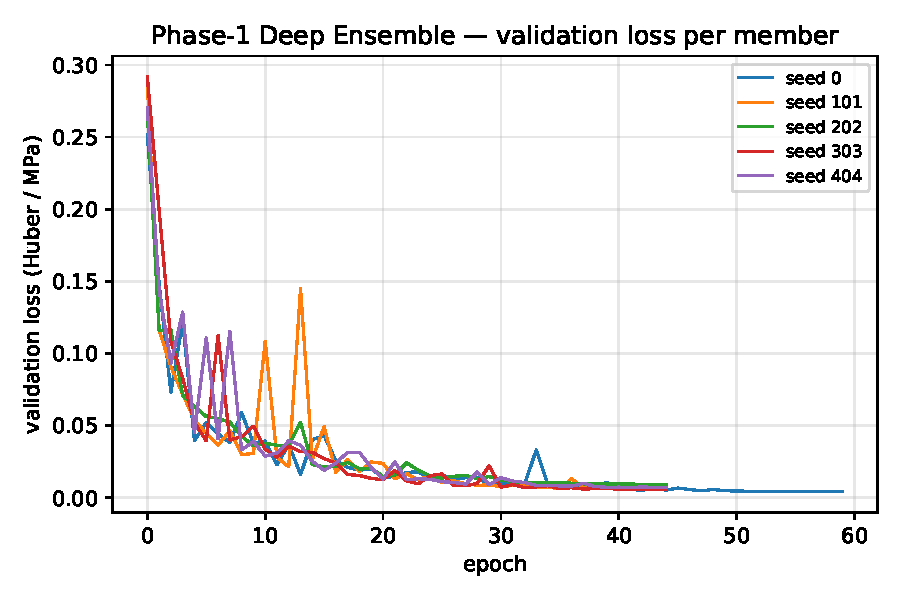
\includegraphics[width=0.75\linewidth]{figures/fig_phase1_training_curves.pdf}
  \caption{Validation loss per epoch for the five Deep-Ensemble members
    (seeds $101,\ldots,505$). Huber loss on the un-normalized stress
    target in MPa; cosine schedule with early stopping patience $12$.}
  \label{fig:phase1-curves}
\end{figure}

Representative predictions in the best, median, and worst test samples,
ranked by per-sample mean absolute error, are shown in
Figure~\ref{fig:phase1-examples}. The fillet region --- the dominant stress
concentrator --- is recovered faithfully across the three quantiles; the
visible residual error is almost entirely concentrated at the fillet arc
and hole rims in the worst sample, which is consistent with the
literature-reported pattern that GNN mesh surrogates lose accuracy in the
tail of the stress distribution~\cite{maurizi2022gnn,gladstone2024gnn}
rather than in the bulk.

\begin{figure}[t]
  \centering
  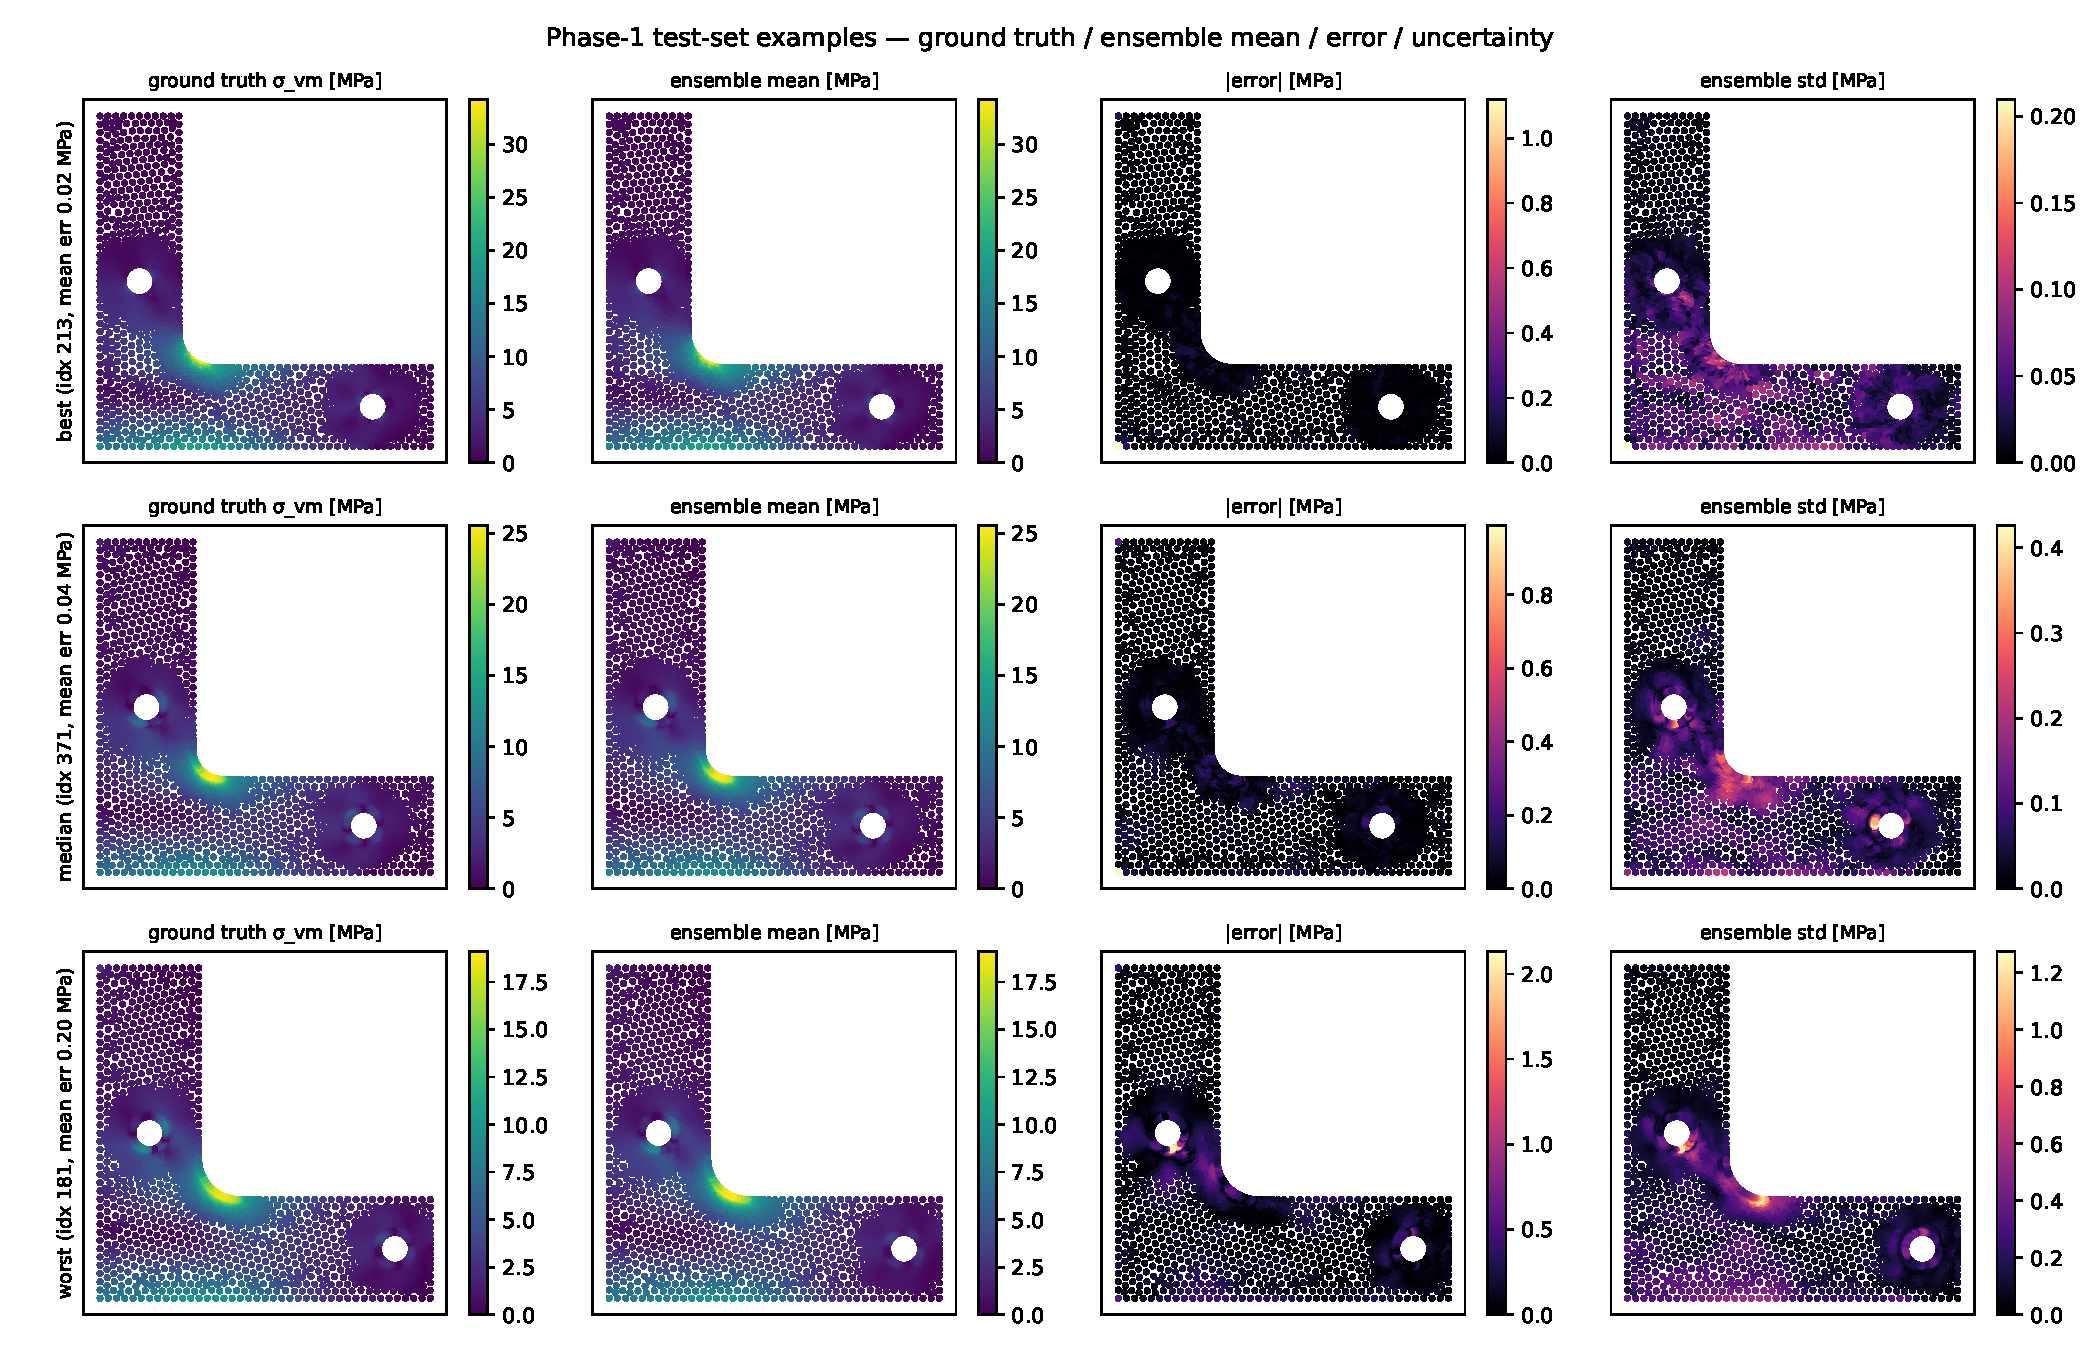
\includegraphics[width=\linewidth]{figures/fig_phase1_example_predictions.pdf}
  \caption{Test-set examples, one row each for the best, median, and
    worst sample by per-sample mean error. Columns, left to right:
    ground-truth von~Mises stress from FEA; ensemble-mean prediction;
    absolute error; ensemble standard deviation (the epistemic-uncertainty
    proxy). The uncertainty map tracks the error map: the GNN knows where
    its predictions are less reliable.}
  \label{fig:phase1-examples}
\end{figure}

\subsection{Ensemble calibration}
\label{ssec:results-calibration}

The central Phase-1 claim is that ensemble disagreement tracks actual
prediction error --- a necessary property for the Phase-2 CQR layer to
operate on a meaningful raw uncertainty signal. We quantify this at two
granularities.

\textbf{Node-level.} Across all $\sim 1.4{\times}10^6$ test-set nodes, we
compute the ensemble standard deviation $s(\mathbf{x}_i)$ and the absolute
residual $r(\mathbf{x}_i) = \lvert \bar{\sigma}(\mathbf{x}_i) -
\sigma^\star(\mathbf{x}_i) \rvert$. The Pearson correlation $\rho_P$ and
Spearman rank correlation $\rho_S$ between these scalars are reported
in Table~\ref{tab:phase1-calibration}; both are materially positive,
confirming that high-uncertainty nodes are also high-error nodes.

\textbf{Sample-level.} Averaging $s$ and $r$ within each test sample
gives a per-sample scatter (Figure~\ref{fig:phase1-calib}, right panel).
This is the deployment-relevant view: a design engineer asks ``for this
candidate bracket, can I trust the surrogate?'' and the ensemble answers
with a sample-level uncertainty. The positive slope is the empirical
foundation for the Phase-2 CQR prediction interval.

\begin{figure}[t]
  \centering
  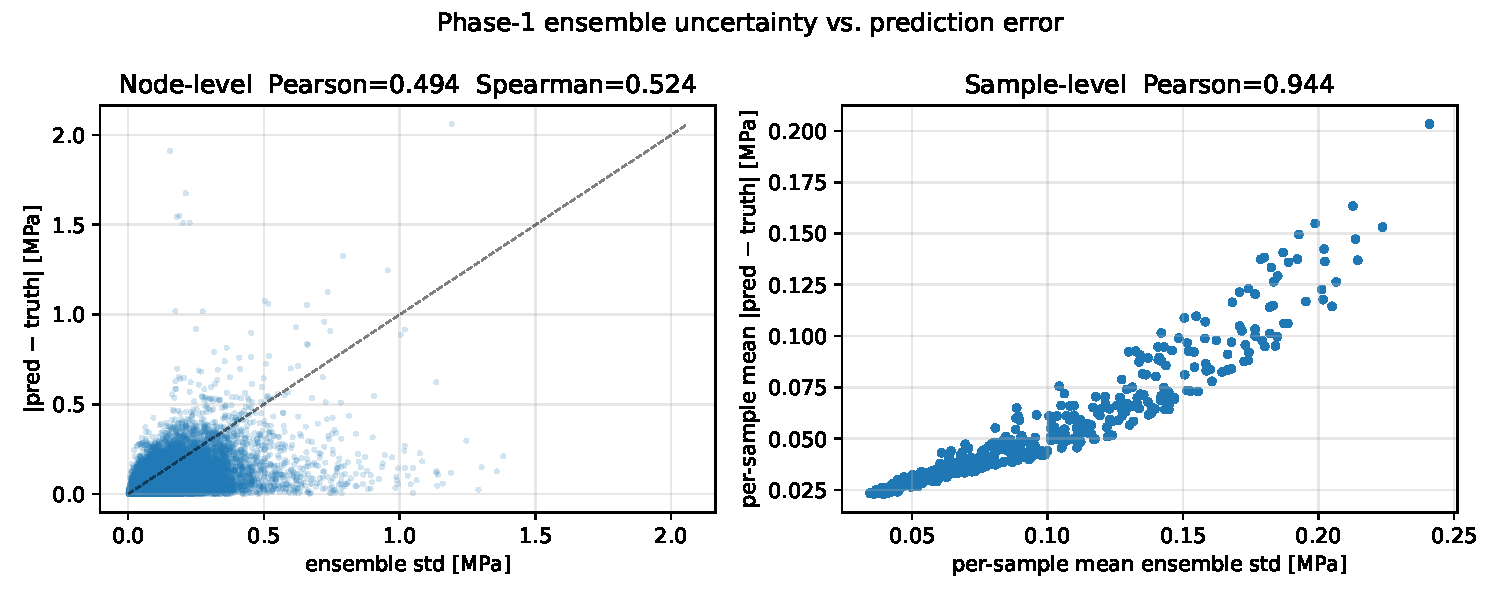
\includegraphics[width=\linewidth]{figures/fig_phase1_calibration.pdf}
  \caption{Ensemble uncertainty (x) vs.\ absolute error (y). \emph{Left:}
    node-level scatter over all test-set nodes. \emph{Right:} per-sample
    scatter with each point representing the mean uncertainty and mean
    error over one test sample.}
  \label{fig:phase1-calib}
\end{figure}

The sample-level correlation specifically is the number to carry forward:
CQR operates on per-sample or per-region scores, not per-node, so the
value reported in Table~\ref{tab:phase1-calibration} sets the headroom
for the coverage-width tradeoff in Phase~2.

\section{Discussion}
% Phase 3: limitations of the reliability layer, failure modes surfaced by OOD, implications for deployment.

\section{Conclusion}
% Phase 3: restate the reliability-layer contribution and calibration guarantees.

\section*{AI Collaboration Disclosure}

This paper was produced in sustained collaboration with AI coding
assistants. Following the precedent set by Matthew Schwartz in the
\emph{Vibe Physics} report, we disclose the AI involvement in scope
and kind rather than attempting to retrospectively excise it.

\paragraph{Session log.}
Every non-trivial decision, deviation from a pre-registered protocol, and
result was recorded to a running session log (\texttt{agent\_log.md} at
the project root) as it happened. That log, not the final code or
figures, is the primary artifact of the human--AI collaboration and is
the raw material for this disclosure.

\paragraph{Orchestrator.}
The end-to-end workflow was driven by Claude Code (Anthropic, Opus~4.7,
1M-context configuration, medium reasoning effort, adaptive thinking
disabled, auto-memory disabled) running locally against the project
repository. The orchestrator wrote the project's Python code (FEniCSx
sweep scripts, PyTorch-Geometric models and training loops, the
conformal-prediction module, analysis scripts, figure generators), drove
the dataset-generation and training compute, and drafted all sections of
this manuscript. A human author directed the orchestrator throughout:
choosing the scientific problem and the reliability-layer framing;
locking the material model, parameter ranges, load calibration, and OOD
protocol at the points marked ``locked'' in the session log before any
model was trained; approving every deviation from the pre-registered
protocol; reading and editing the generated manuscript sections; and
making the publish-or-revise calls at each phase boundary.

\paragraph{Research corpus and retrieval.}
Citation claims in Related Work, Methods, and Discussion were grounded
in the project's on-disk paper corpus (\texttt{raw/papers/}), which was
curated in separate sessions by a different AI assistant (Claude Sonnet
in a documented corpus-curation role) and held read-only with respect to
the orchestrator. The orchestrator used a knowledge-graph retrieval layer
(Graphify) over this corpus at pre-designated decision points during
method design (GNN architecture, ensemble-size justification,
conformal-prediction algorithm and theorem reference, OOD evaluation
practice) to select which prior work to ground each claim on; every
such query and its useful / partial / unused outcome is logged in the
session log.

\paragraph{Code, figures, and numerical results.}
All code in the project repository was written by the orchestrator and
reviewed by the human author before execution on the training and OOD
data. All reported numerical results (per-node MAPE, peak-stress MAPE,
coverage tables, interval widths, per-condition OOD breakdown, deferral
rule operating points) are the direct output of that code on the frozen
datasets and the frozen model artifacts; they were not edited,
hand-tuned, or re-described after generation. Every figure in this paper
is emitted programmatically by a Python script
(\texttt{scripts/phase1\_eval.py}, \texttt{scripts/phase2\_cqr.py},
\texttt{scripts/phase3\_ood.py}) from the cached prediction arrays, with
the exception of the L-bracket illustration (Figure~\ref{fig:bracket_photo}),
which is a human-produced engineering rendering.

\paragraph{Manuscript text.}
The LaTeX source was drafted by the orchestrator from the session log
and the numerical results, and edited by the human author for tone,
scoping, and scientific emphasis. The orchestrator did not have access
to any information beyond the project repository and its curated corpus:
no external web search, no out-of-project knowledge retrieval, and no
re-use of text from prior drafts outside this repository. All
limitations and bounded disclosures (calibration-set reuse, HP-sweep
budget imbalance, ensemble-member epoch differences, plane-stress
idealization, self-weight omission) are present in the manuscript
because the session log required them to be disclosed at the point where
they were incurred.

\paragraph{What the human author contributed.}
The scientific framing (``the contribution is the reliability layer,
not the surrogate''), the choice of study part, the material model, the
load calibration, the $\pm 20\%$ OOD magnitude, the deferral-rule
framing, every ``locked'' pre-registration, every deviation approval,
and the editorial pass on the final manuscript. The human author takes
full responsibility for the scientific content of this paper, including
any errors the AI-generated scaffolding introduced that the editorial
review did not catch.


\printbibliography

\end{document}
